\begin{figure}[htbp]
\centering
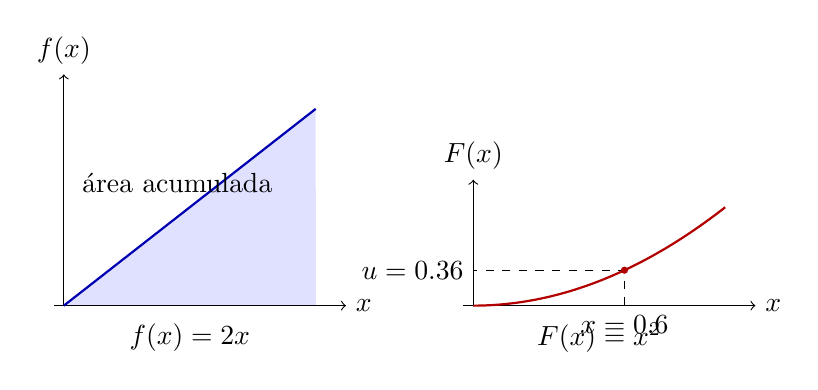
\begin{tikzpicture}[x=3.2cm,y=1.25cm]
  \begin{scope}
    \fill[blue!12] (0,0) -- plot[domain=0:1,samples=50] (\x,{2*\x}) -- (1,0) -- cycle;
    \draw[->] (-0.04,0) -- (1.12,0) node[right] {$x$};
    \draw[->] (0,0) -- (0,2.35) node[above] {$f(x)$};
    \draw[thick,blue!70!black,domain=0:1,samples=50] plot (\x,{2*\x});
    \node[below] at (0.5,-0.08) {$f(x)=2x$};
    \node at (0.45,1.25) {área acumulada};
  \end{scope}
  \begin{scope}[xshift=5.2cm]
    \draw[->] (-0.04,0) -- (1.12,0) node[right] {$x$};
    \draw[->] (0,0) -- (0,1.28) node[above] {$F(x)$};
    \draw[thick,red!70!black,domain=0:1,samples=50] plot (\x,{\x*\x});
    \draw[dashed] (0.6,0) -- (0.6,0.36) -- (0,0.36);
    \fill[red!70!black] (0.6,0.36) circle (1.3pt);
    \node[below] at (0.5,-0.08) {$F(x)=x^2$};
    \node[left] at (0,0.36) {$u=0.36$};
    \node[below] at (0.6,0) {$x=0.6$};
  \end{scope}
\end{tikzpicture}
\caption{La FDA $F(x)=x^2$ integra la densidad $f(x)=2x$. El nivel $u=0.36$ corresponde al cuantil $x=F^{-1}(u)=0.6$.}\label{fig:clase1-densidad-fda}
\end{figure}